\label{chap:analisi}

In questo capitolo vengono presentate le analisi preliminari effettuate per il
caso di studio in questione. Queste analisi hanno permesso di selezionare un
sottoinsieme di job e un task di Machine Learning associato che possa
apportare benefici al CNAF.

\section{Analisi esplorativa}

\subsection{Caratterizzazione dei job}
\label{sec:job_analysis}
In questa tesi considereremo una serie di dati come una sequenza ordinata di
punti dati, che esprime la dinamica di un certo fenomeno nel tempo. Quando
questi dati sono ordinati in base al tempo, si parla di una \textbf{serie
storica} (o \textbf{temporale}).
Indipendentemente dal criterio utilizzato per ordinarli, i punti dati sono
registrati seguendo intervalli di tempo equispaziati. Le serie temporali
possono essere di due tipi: \textbf{univariate}, che coinvolgono una
singola variabile misurata nel tempo, e \textbf{multivariate}, dove più
variabili sono misurate contemporaneamente.

All'interno della tabella \texttt{hj}, che contiene i dati di monitoraggio dei
job eseguiti da HTCondor, ogni riga può essere vista come un punto in una
serie storica multivariata. In altre parole, ciascun job corrisponde a una
serie storica multivariata distinta, dove le variabili rappresentano le
diverse grandezze misurate durante il suo ciclo di vita, come illustrato nella
figura~ \ref{fig:job_time_series}. Sebbene queste serie condividano le stesse
variabili, la durata di ciascun job, e di conseguenza la lunghezza delle
relative serie storiche, cambia.

Come mostrato in figura~\ref{fig:htcondor_sampling}, HTCondor campiona lo
stato di ciascun job ogni tre minuti, ma aggiorna i valori ogni quindici
minuti. Questo significa che ogni serie storica mostra un cambiamento
effettivo nei valori solo ogni cinque campionamenti, risultando in una
sequenza di cinque valori identici che si ripetono fino al prossimo
aggiornamento.

\begin{figure}[p]
    \centering 
    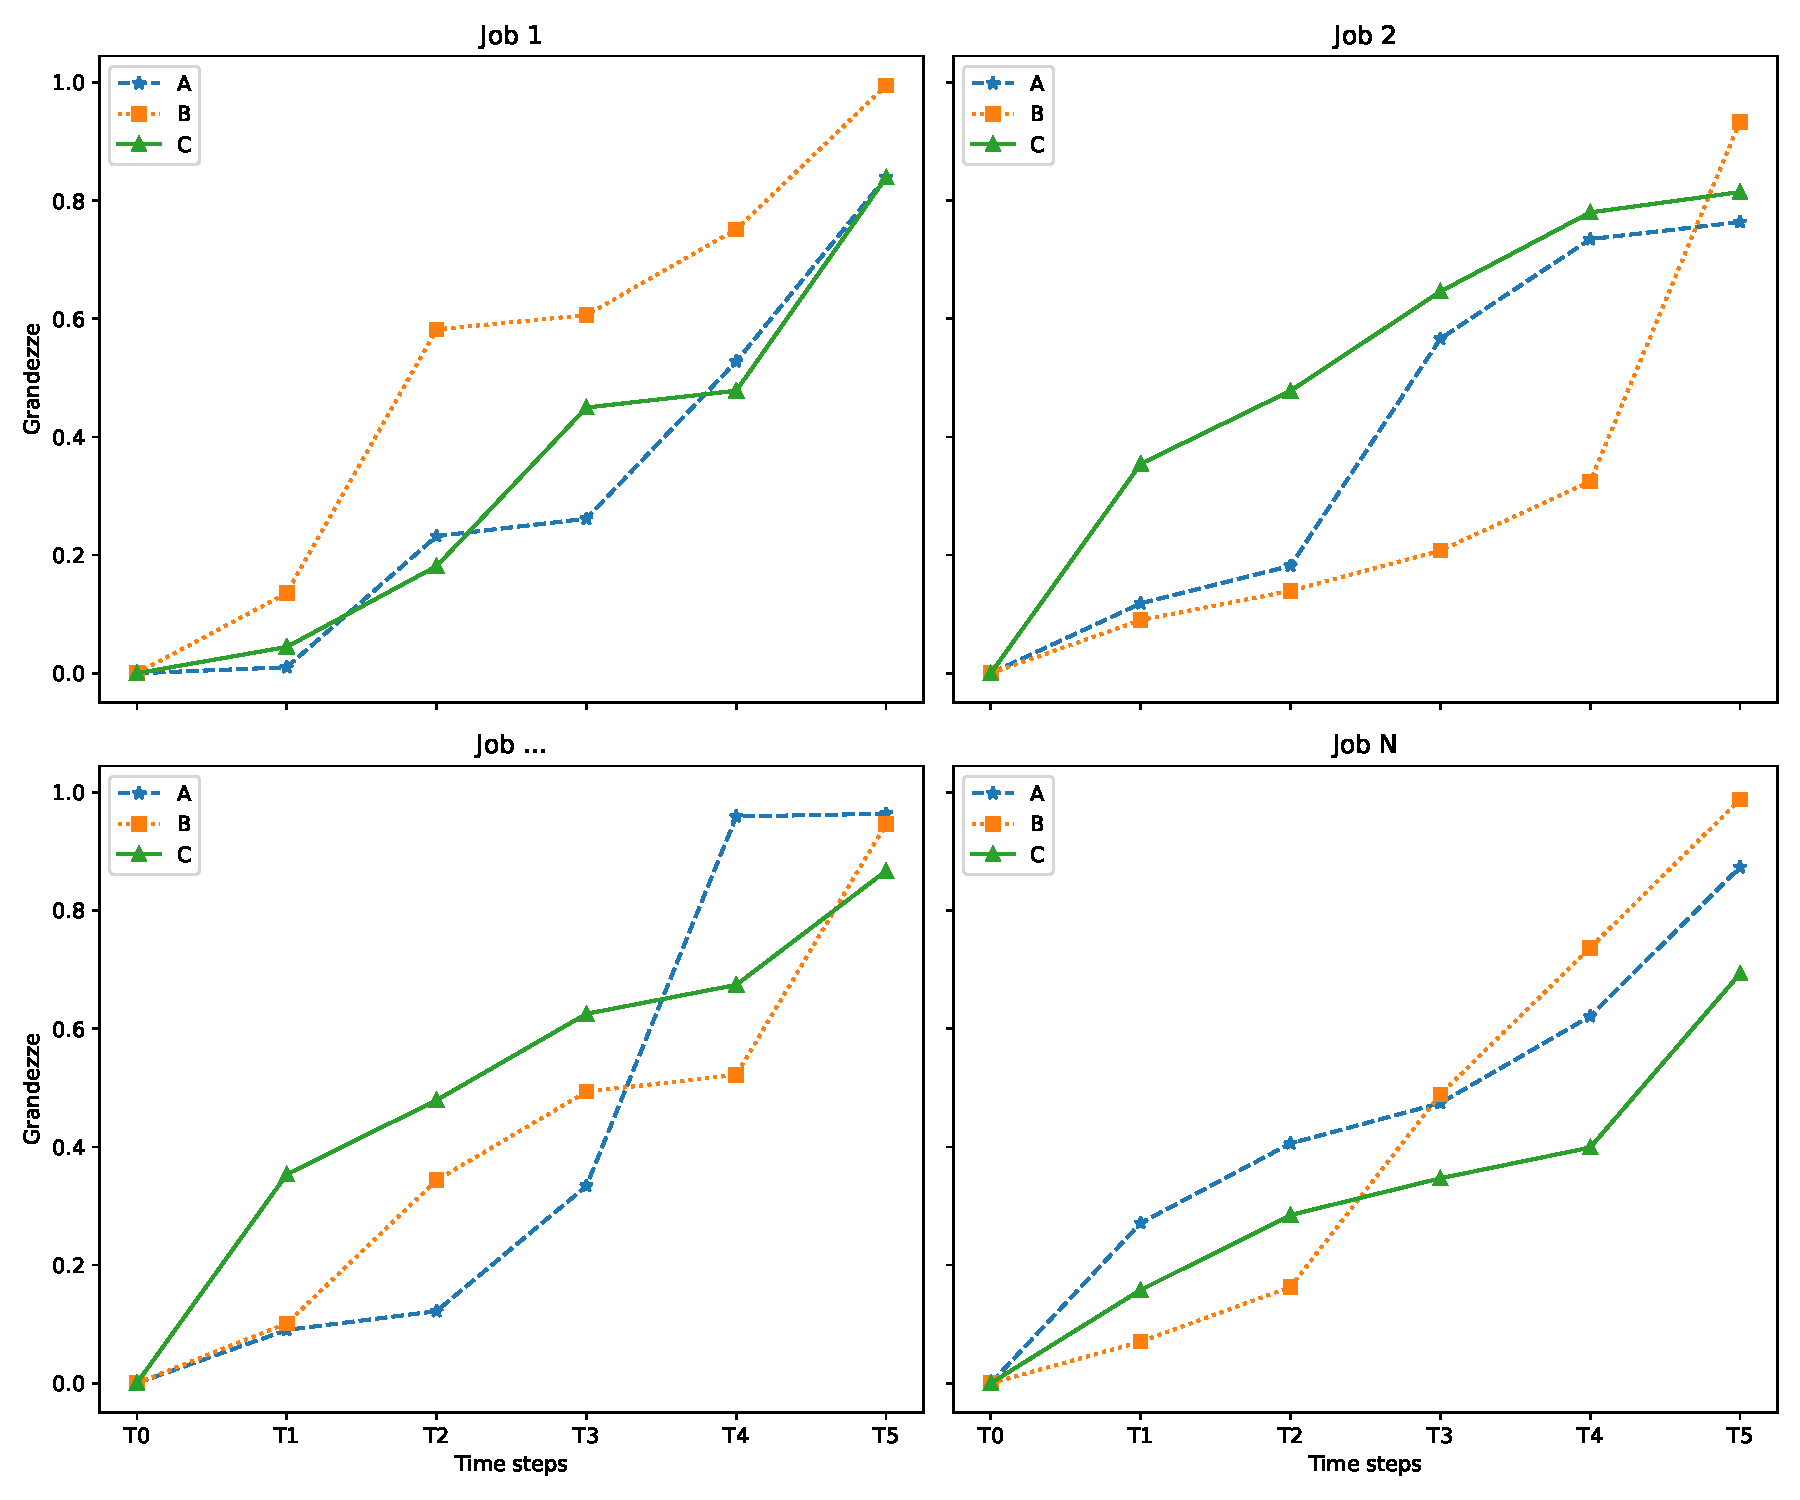
\includegraphics[width=0.95\linewidth]{hj_jobs}
    \caption{\small Rappresentazione di un job come serie storica multivariata}
    \label{fig:job_time_series}
\end{figure}

\begin{figure}[p]
   \centering 
   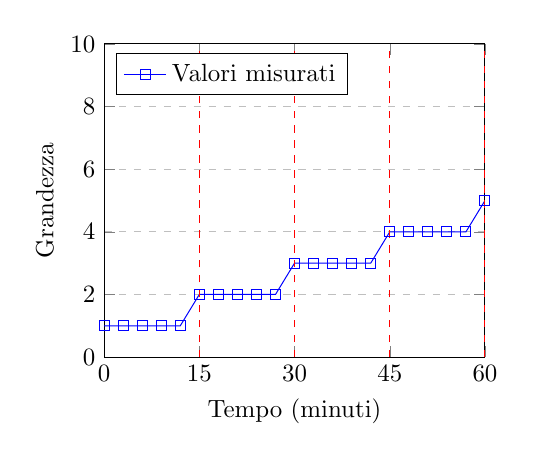
\begin{tikzpicture}[scale=0.9]
       \begin{axis}[
           xlabel={Tempo (minuti)},
           ylabel={Grandezza},
           xmin=0, xmax=60,
           ymin=0, ymax=10,
           xtick={0, 15, 30, 45, 60},
           ytick={0,2,4,6,8,10},
           legend pos=north west,
           ymajorgrids=true,
           grid style=dashed,
           height=6cm
           ]

           % serie storica
           \addplot[color=blue, mark=square]
           coordinates {
               (0,1) (3,1) (6,1) (9,1) (12,1) 
               (15,2) (18,2) (21,2) (24,2) (27,2) 
               (30,3) (33,3) (36,3) (39,3) (42,3) 
               (45,4) (48,4) (51,4) (54,4) (57,4) (60,5)
           };
           \addlegendentry{Valori misurati}

           \draw[dashed, red] (15,0) -- (15,10);
           \draw[dashed, red] (30,0) -- (30,10);
           \draw[dashed, red] (45,0) -- (45,10);
           \draw[dashed, red] (60,0) -- (60,10);
       \end{axis}
   \end{tikzpicture}
   \caption{\small Frequenza di campionamento e aggiornamento dei job in HTCondor}
   \label{fig:htcondor_sampling}
\end{figure}

Per quanto riguarda l'aggiornamento dei valori, HTCondor aggiorna un nuovo
dato all'interno della serie storica solo quando il valore rilevato supera il
precedente massimo. Di conseguenza, ciascuna serie storica può essere vista
come una funzione monotona non decrescente, in cui ogni nuovo valore
registrato è maggiore o uguale al precedente.

La durata dei job varia considerevolmente, come mostrato dalla distribuzione
del numero di job rispetto alla loro durata in giorni, illustrata nella
figura~\ref{fig:job_duration_days}. Vi è una predominanza di job di breve
durata, con un calo esponenziale del numero di job al crescere della durata.

\begin{figure}[!ht]
   \centering
   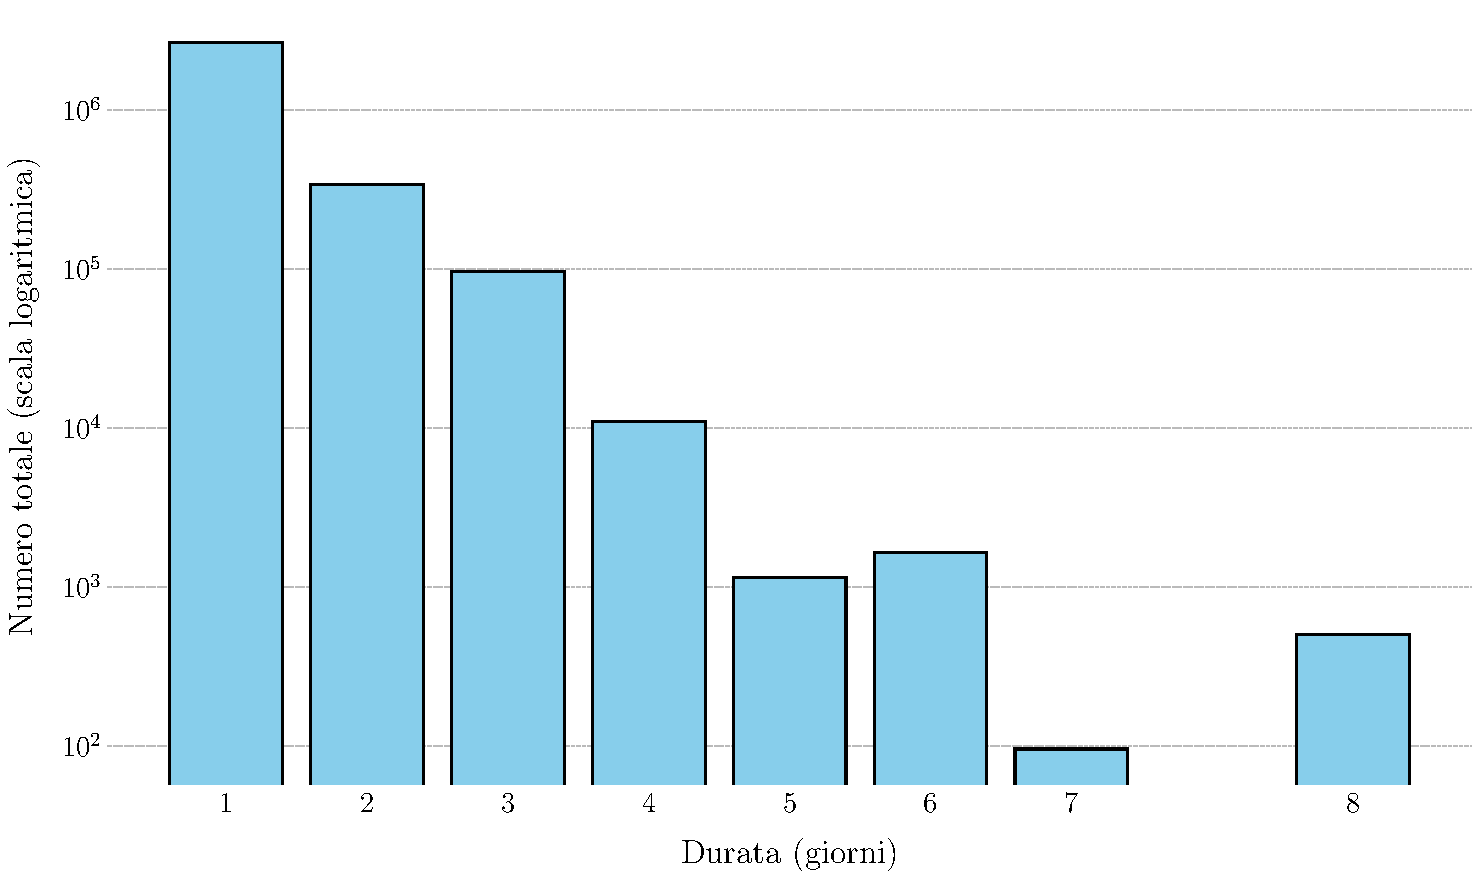
\includegraphics[width=0.85\linewidth]{job_duration_days}
   \caption{Distribuzione della durata dei job in giorni}
   \label{fig:job_duration_days}
\end{figure}

Raggruppando i job in base alla loro durata in fasce orarie, fino a un massimo
di 48 ore, e aggregando tutti quelli che superano tale soglia, è possibile
esaminare il numero totale dei job, la frequenza dei loro fallimenti e il
cumulativo della loro durata per ciascuna delle prime quarantotto ore, così
come per quelli più lunghi. Come evidenziato nella
figura~\ref{fig:njobs_and_rt_perhour}, i job che durano meno di un'ora sono
particolarmente numerosi e presentano un elevato tasso di fallimento.
Nonostante ciò, il tempo speso sulle risorse di calcolo è pressoché
trascurabile se confrontato con il tempo impiegato dai job di durata
superiore.

\begin{figure}[p]
    \centering
    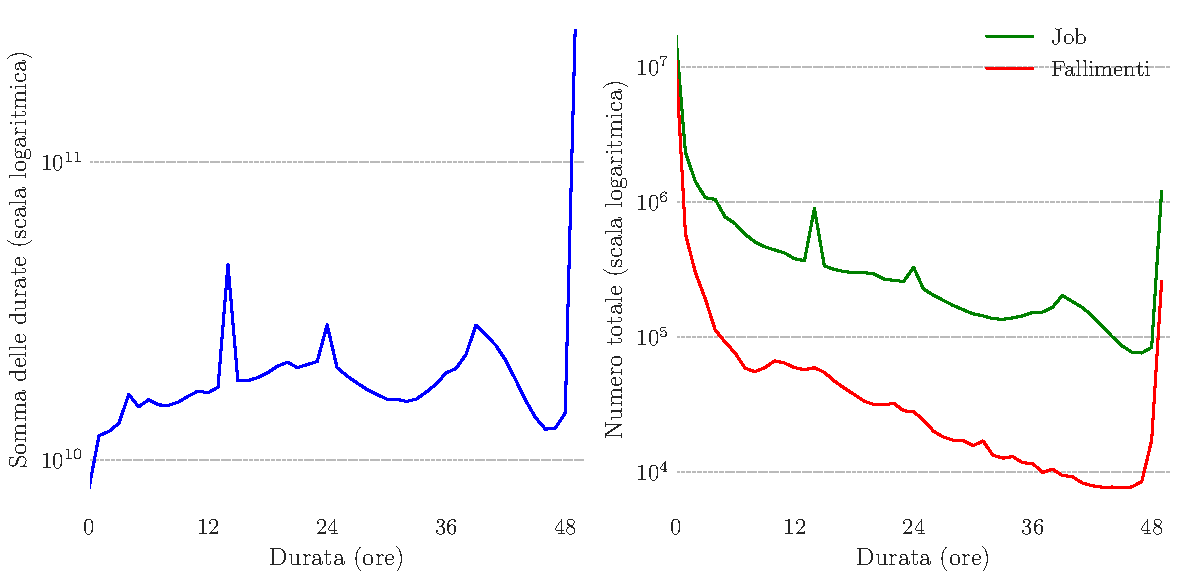
\includegraphics[width=\linewidth]{njobs_and_rt_perhour}
    \caption{\small A sinistra, durata cumulativa dei job; a destra, numero
    totale di job e relativi fallimenti per ogni fascia oraria fino a 48 ore,
mostrati su scala logaritmica}
    \label{fig:njobs_and_rt_perhour}
\end{figure}

Inoltre, se ci focalizziamo sulla prima ora e suddividiamo i job in intervalli
di cinque minuti, possiamo notare che molti di essi hanno una durata inferiore
ai cinque minuti, come si può vedere nella figura~\ref{fig:jobs_firsthour}.
Questo suggerisce che questi job potrebbero essere considerati come semplici
tentativi; in altre parole, sono job che, per vari motivi, non trovano le
condizioni necessarie per proseguire nella loro esecuzione e quindi
falliscono.

\begin{figure}[p]
   \centering
   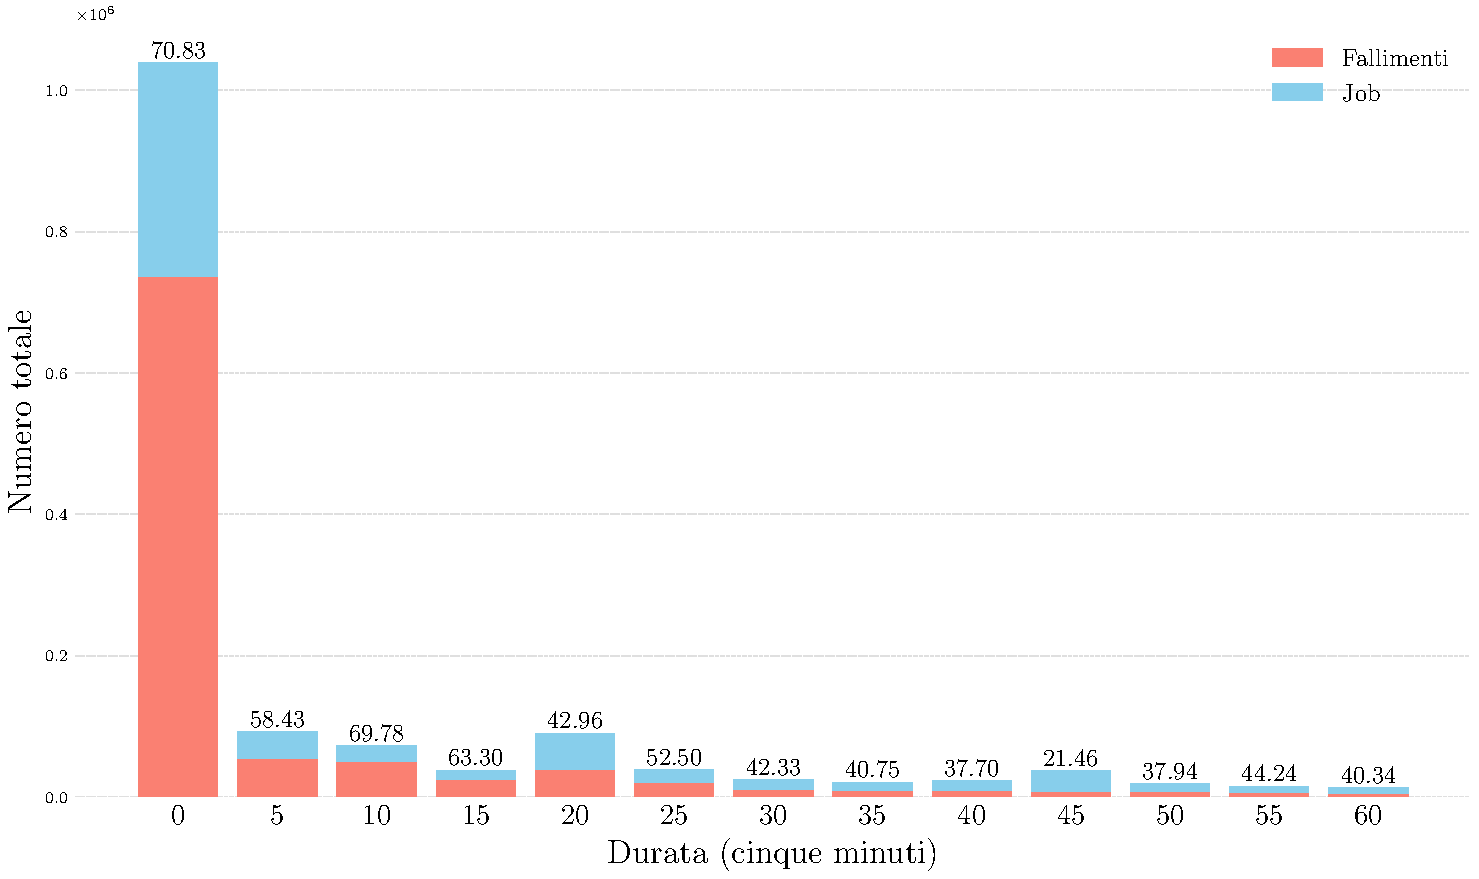
\includegraphics[width=\linewidth]{njobs_firsthour_perfiveminutes}
   \caption{\small Distribuzione dei job nella prima ora, suddivisi in intervalli di
   cinque minuti}
   \label{fig:jobs_firsthour}
\end{figure}

In aggiunta, secondo quanto riportato nella
tabella~\ref{table:pending_jobs_removed}, un significativo 11\% dei job viene
terminato ancor prima di raggiungere la fase di esecuzione. Questi job, non
giungendo alla fase di esecuzione, non effettuano alcun calcolo, il che
sottolinea la presenza di un elevato numero di tentativi che risultano
irrilevanti in termini di calcolo.

\begin{table}[!ht]
    \caption{Percentuale di job in attesa rimossi senza aver effettuato alcun
    calcolo su un host fisico}
    \centering
    \begin{tabular}{ccc}
        \toprule
        \textbf{Job in attesa rimossi} & \textbf{Job eseguiti totali} &
        \textbf{Percentuale} \\
        \midrule
        402,663 & 3,589,280 & 11.22 \\
        \bottomrule
    \end{tabular}
    \label{table:pending_jobs_removed}
\end{table}

Pertanto, alla luce di queste considerazioni, nasce la seguente idea:
\begin{quote}
    \emph{Predire il fallimento di un job di lunga durata è nettamente più
    importante rispetto alla previsione del fallimento di un job di breve durata}.
\end{quote}

\subsection{Caratterizzazione dei gruppi}

L'analisi dei gruppi, come mostrato nella
figura~\ref{fig:job_duration_perqueue}, conferma le osservazioni
precedentemente fatte. La distribuzione della durata dei job per gruppo
riflette l'andamento già notato nella figura~\ref{fig:job_duration_days}. In
particolare, si nota che con l'aumentare dei giorni, il numero di job che
rimangono in esecuzione per quella durata diminuisce esponenzialmente.

\begin{figure}[!p]
    \centering
    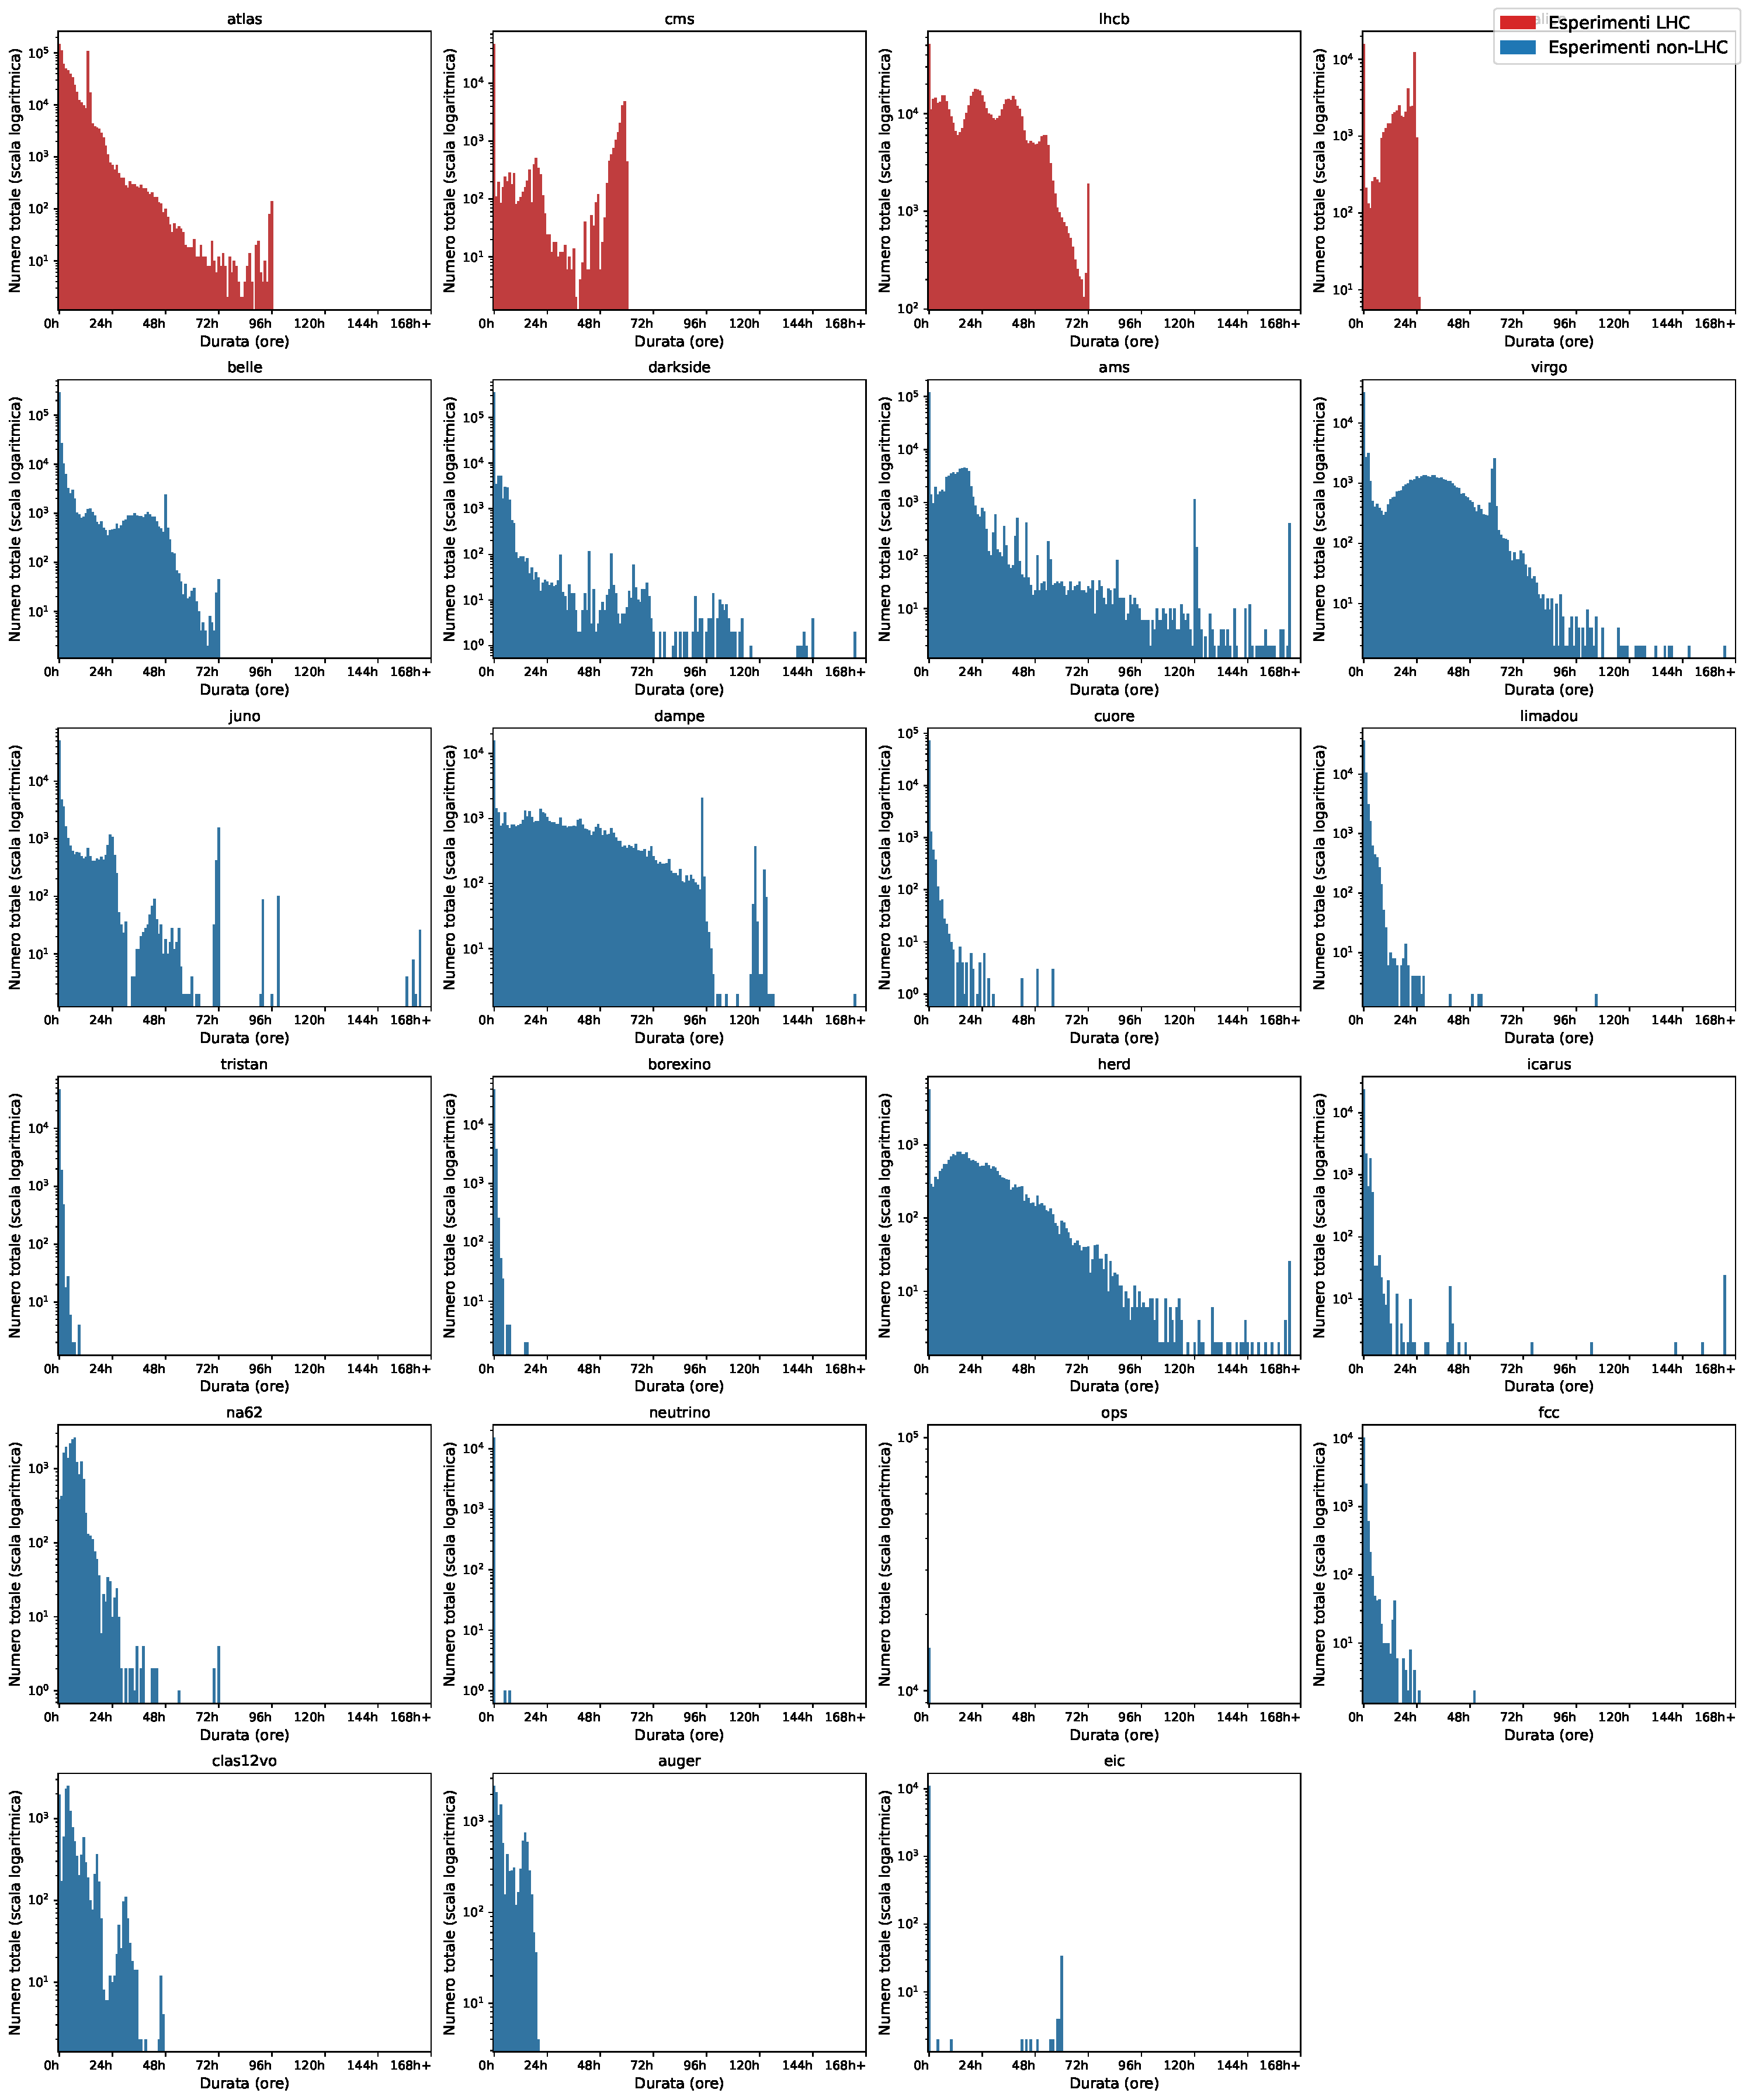
\includegraphics[width=\textwidth]{images/job_duration_perqueue}
    \caption{Distribuzione della durata dei job per gruppo}
    \label{fig:job_duration_perqueue}
\end{figure}

La figura~\ref{fig:njobs_perqueue} evidenzia come i gruppi associati agli
esperimenti LHC sottomettano un numero significativamente maggiore di job
rispetto ai gruppi non-LHC. Questo elevato numero di job, tuttavia, non si
traduce in un tasso di fallimento proporzionalmente alto, come osservato in
precedenza nella figura~\ref{fig:njobs_and_rt_perhour}. Questa differenza può
essere attribuita ai meccanismi interni di controllo presenti nei gruppi LHC,
i quali intervengono rimuovendo autonomamente i job problematici. Al
contrario, alcune code non-LHC presentano un tasso di fallimento estremamente
alto. Tuttavia, le ragioni specifiche di questi fallimenti rimangono a noi
ignote, poiché HTCondor fornisce solo informazioni limitate e generiche sui
motivi dei fallimenti.

\begin{figure}[!ht]
    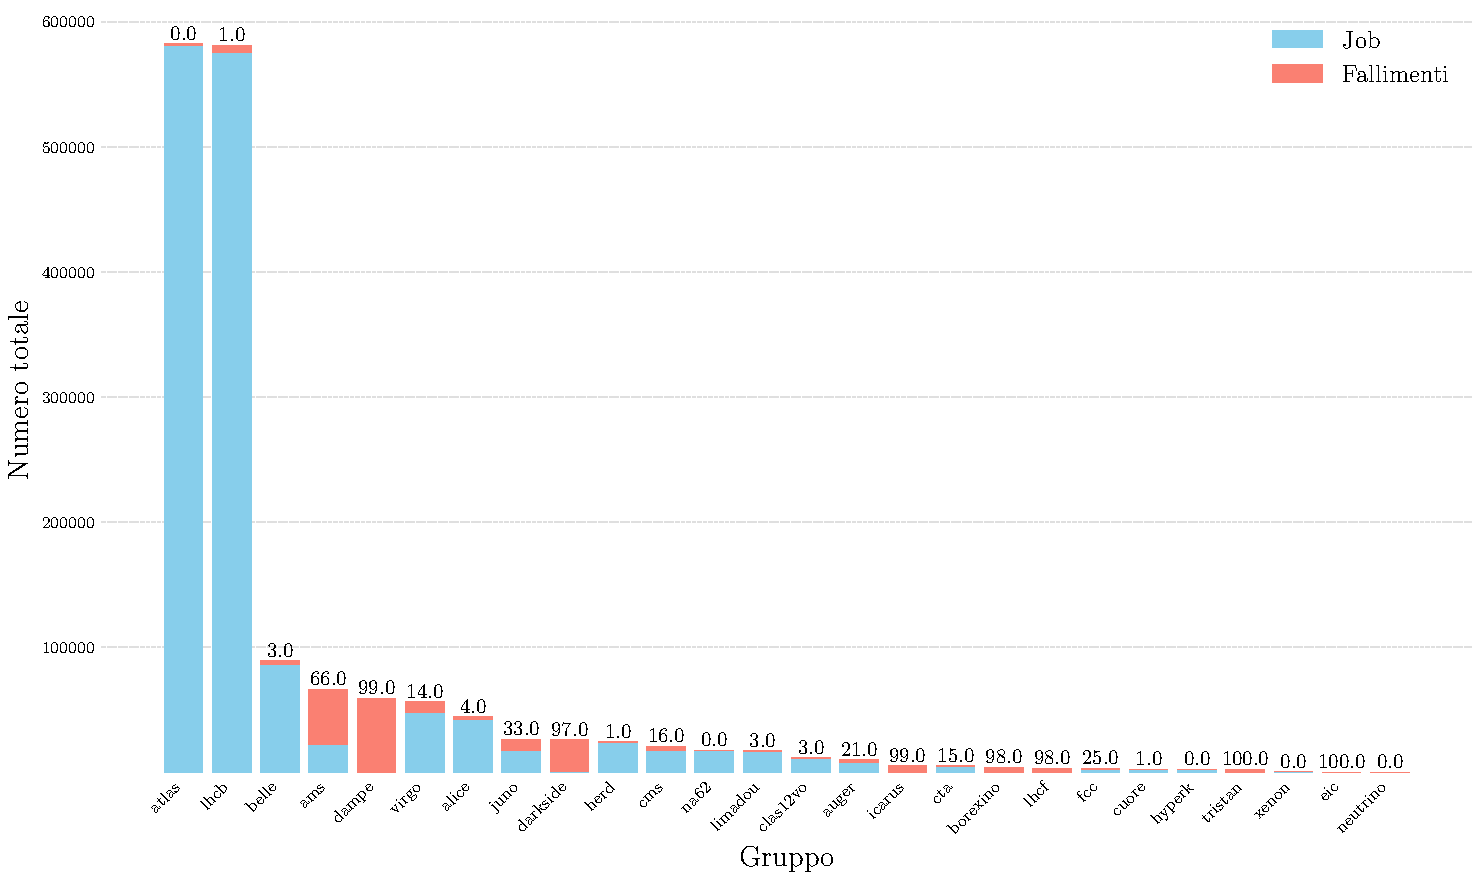
\includegraphics[width=0.95\textwidth]{images/njobs_perqueue}
    \caption{Distribuzione del numero totale dei job e dei loro fallimenti per
    gruppo}
    \label{fig:njobs_perqueue}
\end{figure}

\subsection{Analisi dei nomi dei job}

L'analisi semantica dei nomi dei job può arricchire le feature a disposizione
di un classificatore e migliorarne le prestazioni \cite{Banjongkan2021}. A tal
fine, si sono analizzati i nomi dei job, applicando diverse tecniche di
pulizia del testo per identificare i termini più frequenti.

La tabella~\ref{table:job_names} mostra i risultati dell'analisi semantica
effettuata sui nomi dei job. Questa ha permesso di identificare i cosiddetti
job \texttt{pilot}, i quali sono progettati per insediarsi in un host fisico e
eseguire altri job, detti \texttt{payload}. Questi job non sono direttamente
coinvolti nei calcoli, ma piuttosto servono a scandagliare le risorse
disponibili alla ricerca di un host fisico.

\begin{table}[!h]
    \centering
    \caption{Frequenza dei nomi dei job}
    \begin{tabular}{lr}
        \toprule
        \textbf{Nome} & \textbf{Frequenza} \\
        \midrule
        \texttt{dirac} & 142868 \\
        \texttt{pilotwrapper} & 142868 \\
        \texttt{script} & 72209 \\
        \texttt{eposlhc} & 70736 \\
        \texttt{p5600} & 42766 \\
        \texttt{p100} & 27823 \\
        \texttt{alessr} & 21568 \\
        \texttt{bi210} & 7544 \\
        \texttt{pileup} & 2522 \\
        \texttt{bi214} & 754 \\
        \bottomrule
    \end{tabular}
    \label{table:job_names}
\end{table}

Tuttavia, l'analisi non ha fornito i risultati aspettati. Invece di rilevare
diverse tipologie di job, i nomi tendono spesso a riflettere l'esperimento
scientifico a cui sono associati, informazione meno utile a comprendere le
specifiche funzioni dei job.

\section{Job Zombie Prediction}

Dall'idea delineata nella sezione~\ref{sec:job_analysis}, siamo interessati a
prevedere il fallimento di quei job che garantiscono il maggior payoff. Il
payoff è il beneficio ottenuto, in termini di risparmio di risorse,
interrompendo tempestivamente un job che è destinato a fallire. Rappresentando
il concetto di payoff associato ai job, la figura~\ref{fig:job_payoff}
classifica i job in base alla durata, suddividendoli in tre categorie: corte,
medi e lunghi. È chiaro , come già detto, che interrompere job lunghi sia più
significativo. In questa sezione introduciamo un sottotipo di job lunghi, i
\textbf{job zombie}, la cui interruzione ci può garantire il \textsc{massimo}
payoff.

\begin{figure}[!ht]
    \centering
    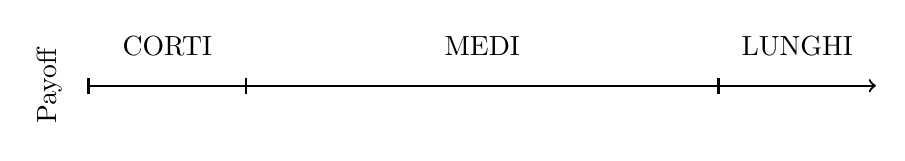
\begin{tikzpicture}
        \draw[thick, ->] (0,0) -- (10,0);
        \draw[thick] (0,-0.1) -- (0,0.1);  

        \draw[thick] (2,0.1) -- (2,-0.1);
        \node at (1,0.5) {CORTI};
        \node at (5,0.5) {MEDI};
        \draw[thick] (8,0.1) -- (8,-0.1);
        \node at (9,0.5) {LUNGHI};

        \node[rotate=90] at (-0.5,0) {Payoff};
    \end{tikzpicture}
    \caption{Rappresentazione dei job in base alla loro durata}
    \label{fig:job_payoff}
\end{figure}

I job zombie sono job che, sebbene ancora in esecuzione, si sono ``bloccati''
a un certo punto della loro attività, cessando di svolgere calcoli utili.
Questi job entrano in uno stato di ``coma'', incapaci di terminare
autonomamente la loro esecuzione e continuano a occupare inutilmente risorse
di calcolo finché, una volta raggiunto il limite massimo di tempo di
esecuzione impostato dal sistema batch, si attiva un evento di timeout che
comporta la rimozione dei job dal sistema. In HTCondor, questo limite è
attualmente fissato a 3 giorni per i job di tipo \texttt{grid} e a 7 giorni
per i job di tipo \texttt{local}.
I job \texttt{local}, sottomessi all'interno della stessa ``farm'' di calcolo
tramite il nodo ``sn-02'' da utenti che fanno parte dell'organizzazione,
beneficiano di maggiore libertà. Al contrario, i job \texttt{grid} vengono
sottomessi tramite nodi, identificati come ``ce0x-htc'', accessibili agli
utenti esterni all'organizzazione.

\begin{table}[!ht]
    \centering
    \caption{Rapporto tra i job zombie e il totale dei job per ciascun gruppo}
    \begin{tabular}{lrrrr}
        \toprule
        \textbf{Gruppo} & \textbf{Job Zombie} & \textbf{Job totali} &
        \textbf{Percentuale} & \textbf{Giorni di calcolo persi} \\
        \midrule
        LHCb & 192 & 262,251 & 0.073\% & 576 \\
        JUNO & 151 & 10,137 & 1.49\% & 453 \\
        ATLAS & 45 & 270,086 & 0.017\% & 135 \\
        LHCf & 8 & 1,594 & 0.502\% & 24 \\
        Belle & 2 & 42,087 & 0.005\% & 6 \\
        \bottomrule
    \end{tabular}
    \label{table:job_zombie_timelost}
\end{table}

La tabella~\ref{table:job_zombie_timelost} mostra un totale di 1,194 giorni di
calcolo persi a causa di job zombie, sottolineando l'entità del problema.
\begin{quote}
    \emph{Un classificatore progettato per identificare precocemente i job zombie
        potrebbe liberare risorse occupate inutilmente da tali job, consentendo a
        nuovi job, potenzialmente produttivi, di iniziare l'esecuzione. Ciò non solo
        ridurrebbe lo spreco di risorse, ma aumenterebbe il throughput del centro di
    calcolo}.
\end{quote}

Purtroppo, poiché HTCondor registra solamente i nuovi massimi nel consumo di
risorse e non tiene traccia dei decrementi, un job zombie potrebbe non
utilizzare più risorse, ma apparire come se le stesse ancora utilizzando.
Questi job possono quindi nascondersi dietro ad altri job che sono in
esecuzione e che stanno utilizzando le risorse, rendendo difficile la loro
identificazione. Questa problematica è confermata nella
figura~\ref{fig:resources_utilization_firstday}: sebbene si osservi il consumo
di RAM, SWAP e disco, la mancata registrazione dei decrementi da parte di
HTCondor non permette di distinguere i job effettivamente in esecuzione da
quelli zombie.

\begin{figure}[p]
    \centering
    \begin{subfigure}[t]{0.8\linewidth}
        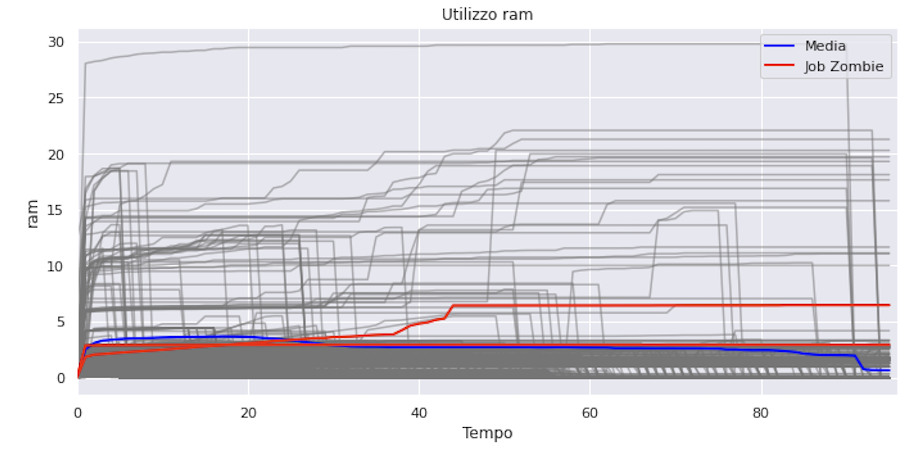
\includegraphics[width=\textwidth]{ram_utilization}
    \end{subfigure}
    \vfill
    \begin{subfigure}[t]{0.8\linewidth}
        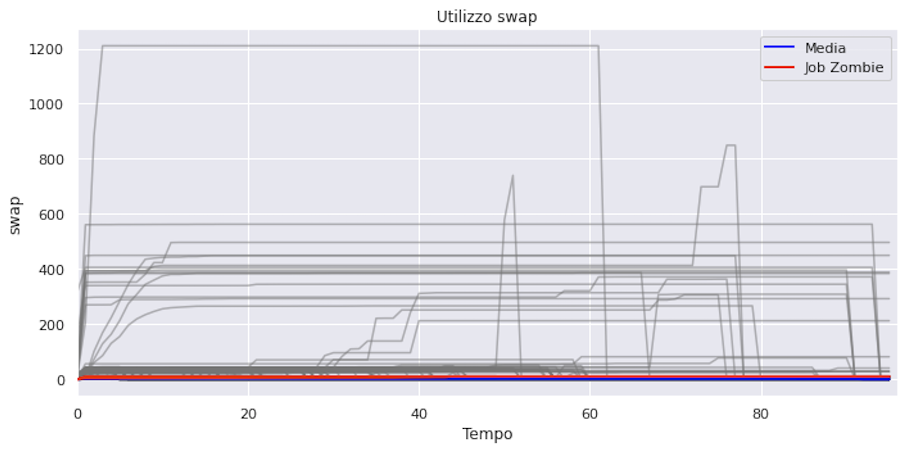
\includegraphics[width=\textwidth]{swap_utilization}
    \end{subfigure}
    \vfill
    \begin{subfigure}[t]{0.8\linewidth}
        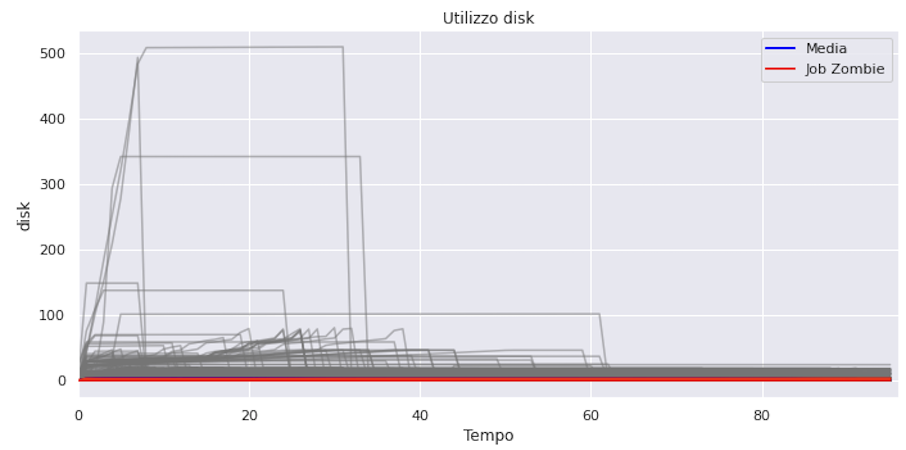
\includegraphics[width=\textwidth]{disk_utilization}
    \end{subfigure}
    \caption{Utilizzo di RAM, SWAP e disco su intervalli di 15 minuti nelle
    prime 24 ore}
    \label{fig:resources_utilization_firstday}
\end{figure}

Un altro problema riguarda la rarità dei job zombie; ad esempio, considerando
i dati di marzo 2023, su un totale di 950,558 job, solo 441 sono job zombie,
corrispondendo a una percentuale dell'appena dello 0,046\%. Questo
sbilanciamento può comportare difficoltà nell'addestramento di classificatori
robusti e porta anche alla necessità di un'estesa raccolta di dati nel tempo.

Per stabilire se l'applicazione di tecniche di Machine Learning è fattibile
nel rilevare i cosiddetti ``job zombie'', è essenziale verificare
preliminarmente la presenza di cluster ben definiti all'interno del dataset.
L'obiettivo sarebbe quello di distinguere con precisione questi job anomali
dagli altri. 

L'algoritmo t-Distribuited Stochastic Neighbor Embedding (t-SNE) consente di
ridurre la dimensionalità dei dati preservando la vicinanza tra i punti simili
e distanziando quelli dissimili \cite{vanderMaaten2008}. Passando da uno
spazio ad alta dimensionalità a uno spazio bidimensionale o tridimensionale è
possibile la visualizzazione dei dati attraverso uno scatterplot.

Tuttavia, t-SNE può essere impraticabile con dataset di grandi dimensioni a
causa della sua complessità computazionale dell'ordine di $\mathcal{O}(N^2)$
\cite{Pezzotti2017}, dove $N$ rappresenta il numero delle istanze. Data la
rarità dei job zombie, è necessario selezionare un ampio periodo di
monitoraggio per raccogliere un campione sufficiente di tali anomalie. Di
conseguenza, si accumula un gran numero di istanze, complicando l'uso di
t-SNE.

Per ovviare a questo problema, si può ricorrere a un'\textbf{autoencoder}, un
tipo specifico di rete neurale progettata per comprimere i dati in una
rappresentazione a dimensionalità ridotta per poi ricostruire un output il più
possibile simile all'input originale. Come illustrato in
figura~\ref{fig:structure_autoencoder}, un autoencoder è composto da due parti:
una funzione di codifica (\textit{encoder}) che trasforma l'input in una
rappresentazione compressa ($h=f(x)$) e una funzione di decodifica
(\textit{decoder}) che ricostruisce l'input a partire dalla rappresentazione
compressa ($r=g(h)$). L'obiettivo è che la rete impari una funzione $g(f(x))$
che non restituisca $x$ ma piuttosto una rappresentazione semplificata
dell'input \cite{Goodfellow2016}.

\begin{figure}[!ht]
    \centering
    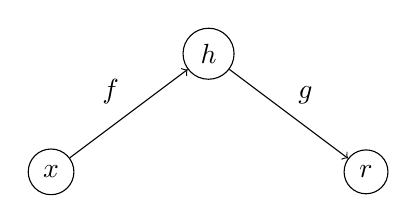
\begin{tikzpicture}
        \node (x) at (0,0) [circle,draw] {$x$};
        \node (h) at (2,1.5) [circle,draw] {$h$};
        \node (r) at (4,0) [circle,draw] {$r$};

        \draw[->] (x) -- (h) node[midway,above left] {$f$};
        \draw[->] (h) -- (r) node[midway,above right] {$g$};
    \end{tikzpicture}
    \caption{Struttura generica di un autoencoder \cite{Goodfellow2016}} 
    \label{fig:structure_autoencoder}
\end{figure}

Se i dati sono caratterizzati da relazioni non lineari, gli autoencoder con
funzioni di codifica e decodifica non lineari sono in grado di modellare e
preservare tali relazioni anche dopo la compressione dei dati in uno spazio a
dimensione ridotta \cite{Goodfellow2016}.

La figura~\ref{fig:tsne_zombiejobs} mostra come, l'applicazione di autoencoder
per la compressione dei dati, seguita dall'analisi t-SNE, ha permesso
l'identificazione di cluster distinti di job zombie accumulatisi nel 2021. È
tuttavia importante prestare attenzione all'interpretazione dei risultati
ottenuti con t-SNE, infatti le distanze tra i cluster o le loro dimensioni
apparenti non sono significative \cite{Wattenberg2016}. In aggiunta, la
composizione di questi cluster risulta indipendente dal gruppo che ha
sottomesso i job. La prevalenza di job provenienti dagli esperimenti LHCb e
ATLAS non riflette altro che l'abbondante sottomissione di job da parte degli
esperimenti LHC.

Ulteriormente, esaminando i job relativi agli esperimenti LHC, in particolare
quelli relativi ad ATLAS, durante la seconda metà di settembre 2021, si è
notato che alcuni job zombie si raggruppano in cluster distinti, come
illustrato nella figura~\ref{fig:tsne_sep2021}. Questo suggerisce che questi
job potrebbero essere identificati con maggiore facilità. D'altra parte, vi
sono job che si mescolano tra quelli normali, il che potrebbe rendere la loro
individuazione più complessa.

\begin{figure}[!hb]
   \centering
   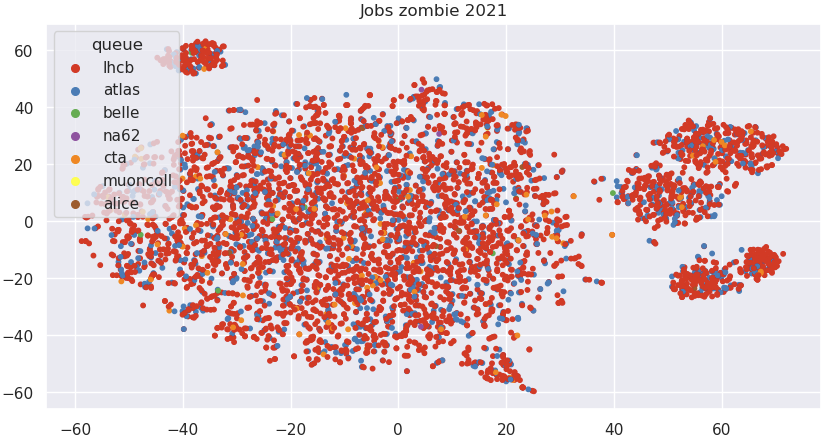
\includegraphics[clip, trim=1.5cm 1cm 0cm 0.75cm, width=0.65\linewidth]{tsne_zombiejobs}
   \caption{Visualizzazione job zombie del 2021 tramite t-SNE}
   \label{fig:tsne_zombiejobs}
\end{figure}

\begin{figure}[!hb]
   \centering
   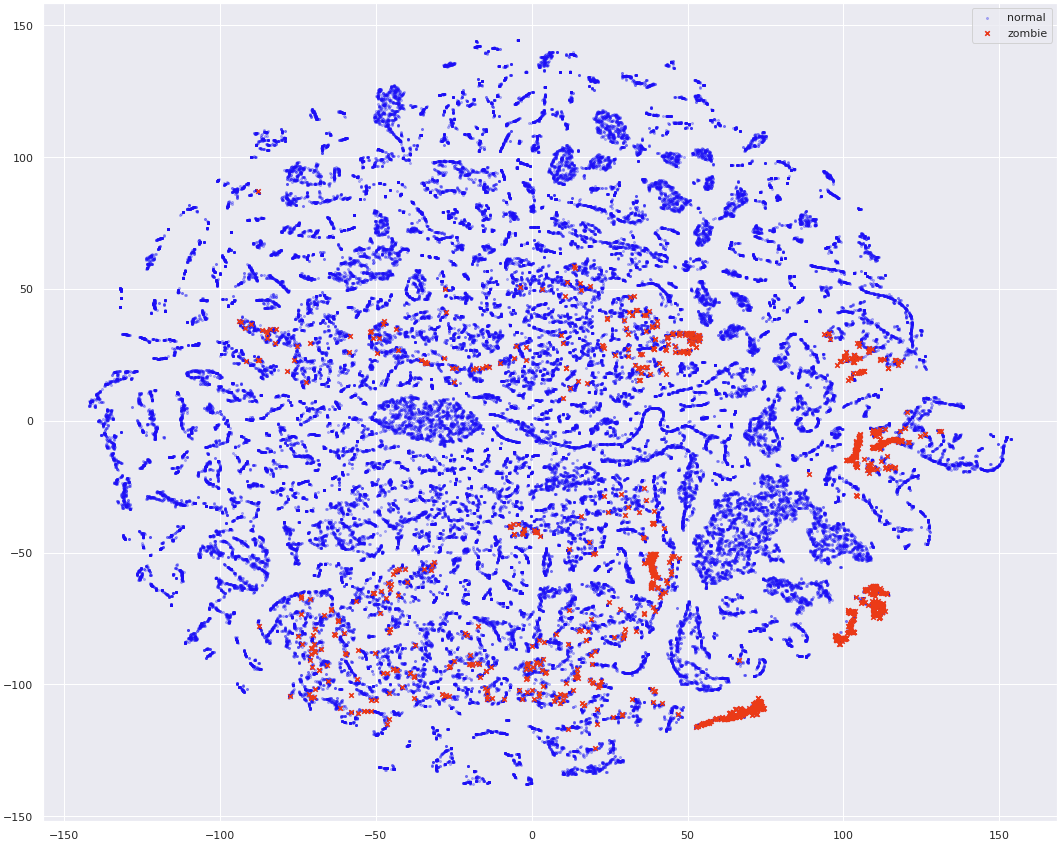
\includegraphics[clip, trim=1.5cm 1cm 0cm 0cm, width=0.65\linewidth]{tsne_sep2021}
   \caption{Visualizzazione job ATLAS di settembre 2021 tramite t-SNE}
   \label{fig:tsne_sep2021}
\end{figure}

In conclusione, 
\begin{quote}
    \emph{l'obiettivo di questa tesi è verificare che i job zombie possano
    essere identificati attraverso l'applicazione di modelli di Machine
Learning.}
\end{quote}

Nel capitolo~\ref{chap:machine_learning}, esploreremo due diversi modi di
modellare il problema con il Machine Learning, applicando tecniche specifiche
per ciascuno. Successivamente, nel capitolo~\ref{chap:valutazioni}, valuteremo
e confronteremo i risultati ottenuti attraverso i due approcci e le relative
tecniche utilizzate.
